В библиотеке \textbf{numpy.fft} есть функция \textbf{fft}, которая реализует быстрое преобразование Фурье. Задается она, согласно документации, следующим образом:
\begin{equation}
    F(k) = \sum_{n=0}^{N-1} f(n) e^{-2\pi i k n / N} x(n)
\end{equation}
И обратное преобразование Фурье \textbf{ifft}:
\begin{equation}
    f(n) = \frac{1}{N} \sum_{k=0}^{N-1} F(k) e^{2\pi i k n / N}
\end{equation}
Для того, чтобы сделать это преобразование унитарным, необходимо 
умножить результат прямого преобразования на $\dfrac{1}{\sqrt{N}}$, а результат обратного преобразования на $\sqrt{N}$.

\subsection{Восстановление функции из ее образа}
\def\steps{1000}
Посмотрим на то, как будет выглядеть восстановленная из образа функции при использовании \texttt{ifft} на рисунке \ref{fig:\steps_ifft_cmp}.
\begin{figure}[ht!]
    \centering
    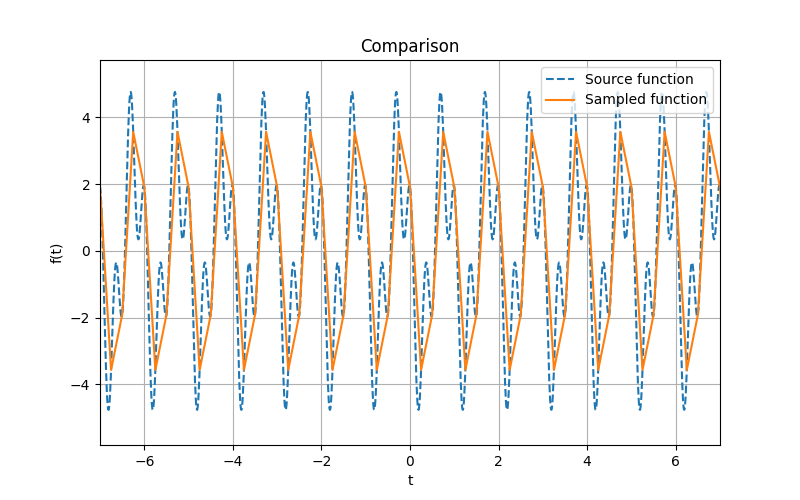
\includegraphics[width=\textwidth]{plots/fft_\steps/cmp_func}
    \caption{Сравнение исходной и восстановленной функции (разбиение на $\steps$ точек)}
    \label{fig:\steps_ifft_cmp}
\end{figure}

На рисунке \ref{fig:\steps_ifft_cmp} видно, что исходная и восстановленная функции не совпадают. 
Посмотрим на график разности исходной и восстановленной функции на рисунке \ref{fig:\steps_ifft_error}.
\begin{figure}[ht!]
    \centering
    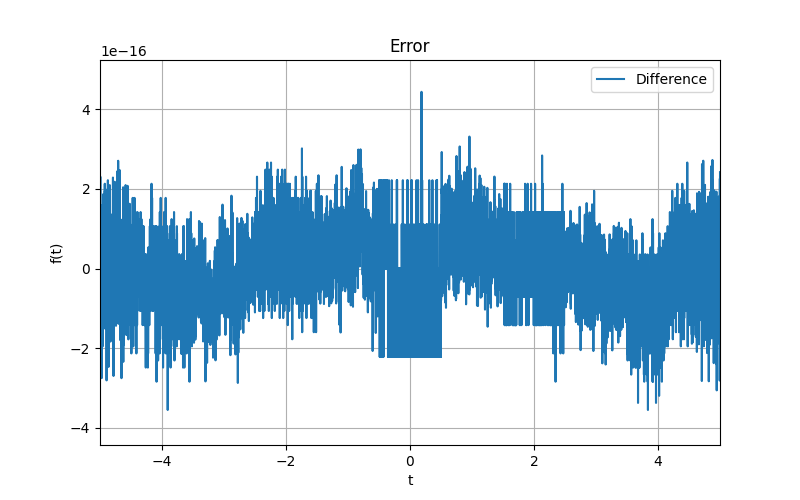
\includegraphics[width=\textwidth]{plots/fft_\steps/error}
    \caption{Разность исходной и восстановленной функции (разбиение на $\steps$ точек)}
    \label{fig:\steps_ifft_error}
\end{figure}

Видно, что ошибка по модулю не превышает $4 \cdot 10^{-16}$, что говорит о том, что восстановленная функция практически идеально совпадает с исходной.
При этом скорость работы алгоритма быстрого преобразования Фурье значительно выше, чем обычного преобразования Фурье.

